\chapter{Introduction}	\label{ch:introduction}
The simulation of combustion processes poses a significant computational challenge due to the intricate interplay between chemical reactions and fluid dynamics. Of particular interest is the simulation of a diffusion flame, which arises from the non-premixed mixing of fuel and oxidizer. The use of numerical methods to simulate a diffusion flame can offer crucial insights into flame structure and combustion efficiency. Discontinuous Galerkin methods are a class of numerical techniques that have demonstrated high accuracy and efficiency for simulating combustion processes. In this thesis, the suitability of Discontinuous Galerkin methods for simulating a diffusion flame will be explored, and the outcomes of the simulations will be analyzed.

\section{The Discontinuous Galerkin method for reacting flows}
The field of \Gls{CFD} has become a crucial tool for understanding and predicting complex fluid flows. With the use of numerical methods and specialized algorithms, CFD allows researchers to simulate fluid dynamics problems and gain detailed insights into the behavior of fluids in motion. Detailed information about flow physics that is often difficult or impossible to obtain through experimental means can be provided by these methods, leading to deeper insights into the mechanisms governing fluid flow. 

In addition to their scientific value, numerical methods for fluid dynamics have numerous practical applications. For instance, the design of devices such as aircraft wings or turbine blades, can be optimized to improve their performance and efficiency. They are also crucial for assessing the safety and reliability of systems such as pipelines or chemical reactors, and identifying potential problems before they occur.

Historically, low-order numerical methods, such as finite difference or finite volume methods, have been commonly used for fluid dynamics simulations. These methods use lower order polynomial functions to approximate the solution of the governing \glspl{PDE}. On the other hand, the so called high order methods use higher order polynomial functions to approximate the solution, allowing them to capture sharp gradients and complex flow structures with greater fidelity. While high-order methods are more computationally expensive than low-order methods, they offer the potential for significantly greater accuracy. 

High-order methods have been used since the early days of numerical simulation, but their use was limited due to their high computational cost. With the advent of modern high-performance computing systems and algorithms, the use of high-order methods has become more widespread and accessible. %The first high-order methods used were based on finite element techniques, such as the Galerkin method, which were used to solve elliptic \glspl{PDE}. In the 1970s, high-order methods based on spectral techniques, such as the spectral element method, were developed. In the 1980s and 1990s, high-order methods based on the finite volume approach, such as the \gls{ENO} and  \gls{WENO} \parencite{liuWeightedEssentiallyNonoscillatory1994}, were developed and used to solve hyperbolic PDEs, such as the Euler equations for compressible fluid flow.

Today, high-order methods are widely used in many areas of computational fluid dynamics, including aerospace \parencite{mavriplisProgessHighOrderDiscontinuous2009}, automotive \parencite{colomboAssessmentDiscontinuousGalerkin2021}, and biomedical engineering \parencite{fehnModernDiscontinuousGalerkin2019}, among others. They continue to evolve and advance, with ongoing research focused on improving their accuracy, robustness, efficiency, and applicability to a wider range of fluid flow problems \parencite{perssonSubCellShockCapturing2006}. One of the most prominent methods is the so-called Discontinuous Galerkin method, which is the subject of this thesis.

\subsubsection{The Discontinuous Galerkin method}
The \gls{DG} method is a numerical method used for solving \glspl{PDE}. It was initially developed for solving hyperbolic conservation laws, and has recently gained increased attention in the \gls{CFD} community. The key feature of the method is the use of a piecewise polynomial approximation of the solution field on each element of a computational mesh. This allows for high accuracy and flexibility, with the order of the polynomial being a tunable parameter. 
The DG method combines the locality of low-order schemes with the accuracy per \gls{DOF} of spectral schemes. This feature allows for achieving the same level of accuracy as a low-order scheme with fewer \glspl{DOF}, leading to more efficient and computationally feasible solutions.  Another advantage of the  DG method is that is well suited to parallel computing. Within the DG method any given cell of the grid only requires information from its immediate neighbours, allowing an efficient parallelization with minimal communication overhead.
lala \gls{DOF} lala \glspl{DOF}

Additionally, within the DG method, the solution is allowed to be discontinuous across element boundaries, which allows for the treatment of complex geometries and discontinuities in the solution. It is worth noting that the conservation of a physical quantity (such as mass, momentum, or energy)  is ensured  in the DG method. This is achieved through the use of numerical fluxes, which approximate the flux of the conserved quantity at each element boundary. The numerical fluxes must meet certain stability and accuracy criteria to ensure the overall stability and accuracy of the method. 

%Additionally, the DG method is capable of handling under-resolved flows \parencite{henninkLowMachNumberFlow2022}. 

%\subsubsection{How does the Discontinuous Galerkin method compare to other methods?}
Compared to more classical and well known methods, such the \gls{FEM} and \gls{FVM}, the DG method has several advantages. First, The DG method provides an arbitrary order of error convergence through the local polynomial approximation of the solution field. Specifically, a polynomial approximation of degree $p$ can achieve a numerical discretization error of order $\mathcal{O}(h^{p+1})$ for smooth solutions, where $h$ is a characteristic grid length. In contrast, the \gls{FVM} is often restricted to accuracy of $\mathcal{O}(h^N)$, with $N \leq 2$ for unstructured grids. Second, the discontinuous approximation of the solution in the DG method allows for the treatment of discontinuities in the solution, which can be challenging for the classical \gls{FEM}. Additionally, the DG method is better suited for solving problems with complex geometries and non-conforming meshes. 

 On the other hand, the DG method has the disadvantage that usually the memory requirements  and overall computational costs are higher than a finite element method.


\subsubsection{Diffusion flame modelling and the Discontinuous Galerkin method}
Diffusion flames, also known as non-premixed flames, pose a significant challenge for simulation due to their complex nature. These flames involve the mixing of two or more reactants before combustion can occur, leading to a complex interplay of fluid dynamics, heat transfer, and chemical reactions. Moreover, diffusion flames are characterized by steep gradients in temperature, density, and species concentration, which can require a high spatial resolution for accurate simulation. The reactants in a diffusion flame are initially separated, and mixing is crucial for combustion to occur. High order methods, such as the DG method, can help alleviate the computational burden associated with the high numerical resolution needed in combustion applications.
 
Representing the chemical reactions involved in the combustion process accurately and efficiently poses a significant challenge. Although a detailed description of the chemistry is preferred, it can be computationally intensive and impractical. To overcome this issue, simplified kinetic models have been developed, such as the one presented by \textcite{fernandez-tarrazoSimpleOnestepChemistry2006} for hydrocarbon combustion with air. This model correlates kinetic parameters with the equivalence ratio, allowing for better representation of the characteristic flame properties of premixed and non-premixed flames. By using a single chemical equation, this model enables the study of complex combustion phenomena while substantially reducing the computational cost. Furthermore, it offers a straightforward and flexible approach to representing phenomena that would otherwise require a more complex chemical model, such as flame temperatures, near-extinction diffusion flames, and reactant leakage.
 
Many practical applications of diffusion flames involve deflagration flames, which are a type of combustion defined by a small characteristic flow velocity compared to the speed of sound.  \parencite{poinsotTheoreticalNumericalCombustion2005}. To accurately model this type of system, the low-Mach approximation of the Navier-Stokes equations is often used. This approximation allows for the calculation of non-constant density flows while neglecting acoustic effects, which reduces the required temporal resolution. 

Explicit time marching algorithms are commonly used for simulations of deflagration flames using the low-Mach approximation, which enables a larger time step size and reduces computational time. However, it should be noted that implicit schemes can also be useful for simulating diffusion flames \parencite{mullerLowMachNumberAsymptoticsNavierStokes1998}. 
\subsubsection{Solution of the system of governing equations}

There are different solution strategies that exist for solving the system of differential equations that govern fluid flow problems. Two common approaches are segregated and fully coupled methods.

In a segregated approach, the equations for each variable are solved separately in a sequence, with the solution of one variable used as input for the solution of the next variable.  The \gls{SIMPLE} algorithm is a popular segregated strategy for solving the discretized system of equations arising in computational fluid dynamics. Originally developed by Patankar \parencite{patankarNumericalHeatTransfer1980} using the \gls{FDM}, the SIMPLE algorithm has proven to be effective in solving a wide range of fluid flow problems. However, as other numerical methods have gained popularity, the SIMPLE algorithm has been extended to work with other discretization methods. For instance, Ferziger and Perić \parencite{ferzigerComputationalMethodsFluid2002} extended the SIMPLE algorithm to work with the \gls{FVM}, while Haroutunian et al. \parencite{haroutunianSegregatedFiniteElement1993} extended it to work with the \gls{FEM}. These extensions have allowed the SIMPLE algorithm to remain a popular choice for solving fluid flow problems, regardless of the numerical method used. The Department of Fluid Dynamics at TU-Darmstadt has developed an extension of the SIMPLE algorithm using the DG method, which was presented in \textcite{kleinHighorderDiscontinuousGalerkin2015}.

Also non-segregated solvers exist. A possibility is the use of fully-implicit Methods. There, the entire system of equations is solved together, rather than being broken down into smaller, independent equations. This means that each equation in the system depends on all the other equations. Fully implicit methods tend to be more robust than segregated methods, as they are less prone to convergence problems or oscillations, especially for problems with complex or nonlinear physics. They present the disadvantage that usually they are more computationally expensive.

When solving fluid flow problems, the discretization of the governing equations typically results in a system of equations that needs to be solved. Nonlinear systems of equations are common in fluid flow problems, and iterative methods such as Picard iteration and Newton's method are often used to solve them. While both methods are iterative and designed for solving nonlinear systems, they differ in their approach to updating the solution at each iteration, as well as their computational cost and convergence properties.

Picard iteration is an iterative method used to solve nonlinear equations by linearizing them. In this method, the nonlinear equation is replaced with a linear equation that approximates the solution around a known solution. This known solution is usually an initial guess or an approximation from a previous iteration. The linearized equation is then solved for the new solution, which is used as the known solution in the next iteration. 

On the other hand, Newton methods are more complex and computationally expensive than picard iteration methods, but they typically converge faster and more reliably. Newton methods involve using the first derivative (Jacobian) of the equations to update the solution in each iteration, which is not always available. Furthermore, the classical Newton method relies on the assumption that the solution is near the initial guess, and may converge slowly or fail to converge if the initial guess is far from the true solution. Globalized Newton methods address this limitation by using a globalization strategy that helps the method to converge to the true solution even if the initial guess is far from it.
 
\section{Objectives and motivation}


In the present work, a low-Mach pressure-based solver for the simulation of temperature dependent non-reactive and reactive flows using the Discontinuous Galerkin method is presented. To the best of the authors knowledge, this is the first time that a pressure-based solver is used together with the DG method for solving the low-Mach equations using a Newton method in a fully coupled manner. While the current study focuses on two-dimensional configurations, the presented concepts could potentially be extended to three-dimensional systems.

This study employs the one-step combustion model proposed by \textcite{fernandez-tarrazoSimpleOnestepChemistry2006} to describe the chemical reactions. While the present work only considers methane combustion, the one-step model could be applied to other hydrocarbons as well. The discrete system of equations is solved using a globalized Newton method with the Dogleg approach. Additionally, the study presents a homotopy strategy that has proven effective in obtaining solutions for highly nonlinear problems in steady-state calculations.

In order to find appropriate initial values for Newton's method in combustion applications, the concept of flame sheet estimates (i.e. the solution for infinitely fast chemistry) is used. Several benchmark cases are presented that allow us to validate our implementation. First we solve the differentially heated cavity problem, with which we intend to validate our implementation of the low-Mach solver for non-constant density flows using the fully coupled solver. Later two flame configurations are calculated, namely the counter-diffusion flame and the chambered diffusion flame. \parencite{matalonDiffusionFlamesChamber1980}
%%%%%%%%%%%%%%%%%%%%%%
In one of the early stages of the implementation of the low-Mach solver the SIMPLE algorithm was adopted for the solution of the velocity-pressure coupling of the governing flow equations. Although this strategy was able to solve various variable density test-configurations, it was observed that the computation times were under certain conditions very high. The solution method includes the use of fixed point iterations, which often require the use of under-relaxation factors, which if not well chosen can dramatically increase the computation time. This was the main motivation for the development of the present solver, which from this point on will be called \gls{XNSEC}. The term \textit{extended} refers to the framework on which the solver is built, which focuses on applications for multi-phase flows using a sharp interface approach using a level-set method. 

The strategy proposed in the present work proposes a fully coupled solution of the system of equations. The non-linear system is solved using a Newton algorithm, and the associated linear problems are solved with a dedicated software (PARDISO). As an example that motivates the development and use of the \cref{fig:RuntimeComparisonk2} strategy, a comparison of the computation times for the same case using a fully coupled approach (XNSEC) and the SIMPLE algorithm is shown 

\begin{figure}[h]	
	\centering
	\inputtikz{RuntimecomparisonWithSimple_k2}
	\caption{Runtime comparison of the DG-SIMPLE solver and the XNSEC solver on a typical simulation.}
	\label{fig:RuntimeComparisonk2}
\end{figure}
Although both algorithms allow the simulation of low-Mach number flows, clearly the SIMPLE algorithm requires much more time. This is by no means an indication that the resolution using a fully implicit scheme is in general superior to a strategy such as the SIMPLE algorithm in the context of DG-methods, and possibly further optimization of the segregated algorithms could lead to an improvement in computation times.




\section{Outline of the thesis}

The thesis is structured as follows: In \cref{ch:gov_eqs} the low-Mach number Navier-Stokes set of equations is presented. The chapter begins by presenting the governing equations in a general way, and concisely shows the main elements for the derivation of the low Mach equations, emphasizing the assumptions made to arrive at them, as well as the models for the different parameters involved in the simulation. In addition, the chemical model chosen for the combustion simulation is presented. Later in \cref{sec:FlameSheet} the concept of the flame-sheet and the Burke-Schumann limit, which are used within the solution algorithm for combustion cases, is shown. 

In \cref{ch:NumericalMethods} the numerical method used in this work is presented. First, a brief introduction to the DG-method is given using a simple transport equation, which allows demonstrating the procedure used for the spatial and temporal discretization of the governing equations. Then in \cref{ssec:nonLinearforms} a description of each of the discretized terms of the governing equations is shown, with special emphasis on the numerical fluxes involved.

The methods for solving the system of discretized equations are presented in \cref{ch:CompMethodology}. The chapter starts with a description of the solver structure, showing the basic building blocks of it. In \cref{sec:SolNonLinProblem} the globalized Newton method used to solve the fully coupled non-linear system is shown. Emphasis is placed on the basic functioning of the method, as well as on certain computational aspects that allow for a higher efficiency. Additionally, in \cref{sec:ConvSupportStrat} additional strategies are presented that improve the convergence properties of the method for cases where the newton algorithm is not able to obtain solutions, such as the use of the flame-sheet estimates for combustion simulations and homotopy methods for highly non-linear problems.

In \cref{ch:results} a comprehensive testing of the solver using a variety of test cases is presented. These test cases are compared with benchmark results, but are also used for highlighting the algorithms introduced in this work. The test cases presented are subdivided in three sections, in increasing level of complexity. First, in \cref{sec:SingleCompIsotCase} the solver is used to calculate typical incompressible benchmark cases, such as lid-driven cavity flow or a backward-facing step, and the results are compared with benchmark solutions. Then in \cref{sec:SinCompNonIsothermCase} the tests are extended to low-Mach number flows, and several typical configurations are calculated for such systems, in particular problems where the temperature has an influence on the flow field, such as the heated square cavity configuration (\cref{ss:DHC}), and the Rayleigh-Bénard Convection problem (\cref{ssec:RayBer}).
Finally in \cref{sec:MultCompNonIsothermCase} the fully coupled system of equations for reactive low-Mach flows is used for calculating some typical diffusion flame configurations. In \cref{ssec:coflowFlame} a coflow flame configuration is simulated. Later in \cref{ss:CDF} a planar counterflow flame configuration is calculated, and the results are compared with simulations of a one-dimensional configuration. 

Finally, a conclusion of the work is done in \cref{ch:conclusion}.


Many parts of the present thesis are based on \textcite{gutierrez-jorqueraFullyCoupledHigh2022}, which has been published by the author of this work.


\section{The BoSSS code}
The presented solver is embedded in the \gls{BoSSS} code, which is under active development at the chair of fluid dynamics of the Technical University of Darmstadt, and is available under \href{https://github.com/FDYdarmstadt/BoSSS}{https://github.com/FDYdarmstadt/BoSSS}.

BoSSS is a general framework for the discretization of conservation laws using the DG method and uses a modal DG approach with orthonormal Legendre polynomials as basis functions. The BoSSS code features a variety of applications in the context of computational fluid dynamics, such as a solver for multiphase flows with a sharp interface approach \parencite{kummerExtendedDiscontinuousGalerkin2017}, an incompressible Immersed Boundary Method solver for particle laden flows \parencite{krauseIncompressibleImmersedBoundary2017}, a solver for viscoelastic fluid flows\parencite{kikkerFullyCoupledHighorder}, and a solver for compressible flows \parencite{geisenhoferDiscontinuousGalerkinImmersed2019}, among others.

The structure of the BoSSS framework is shown in a schematic way in \cref{Fig:BoSSS}. BoSSS allows the end user to develop sophisticated solvers at a very low coding effort. The implementation makes extensive use of several \gls{MPI}-parallel, performance-optimized operations, among which the evaluation of the DG operator can be highlighted, as well as a solution using parallelized algorithms for the resolution of linear systems arising from the discretization. In addition, the user has at his disposal a large number of tools that optimize the workflow, such as the use of Jupyter-notebooks, as well as various post-processing tools.
\begin{figure}
	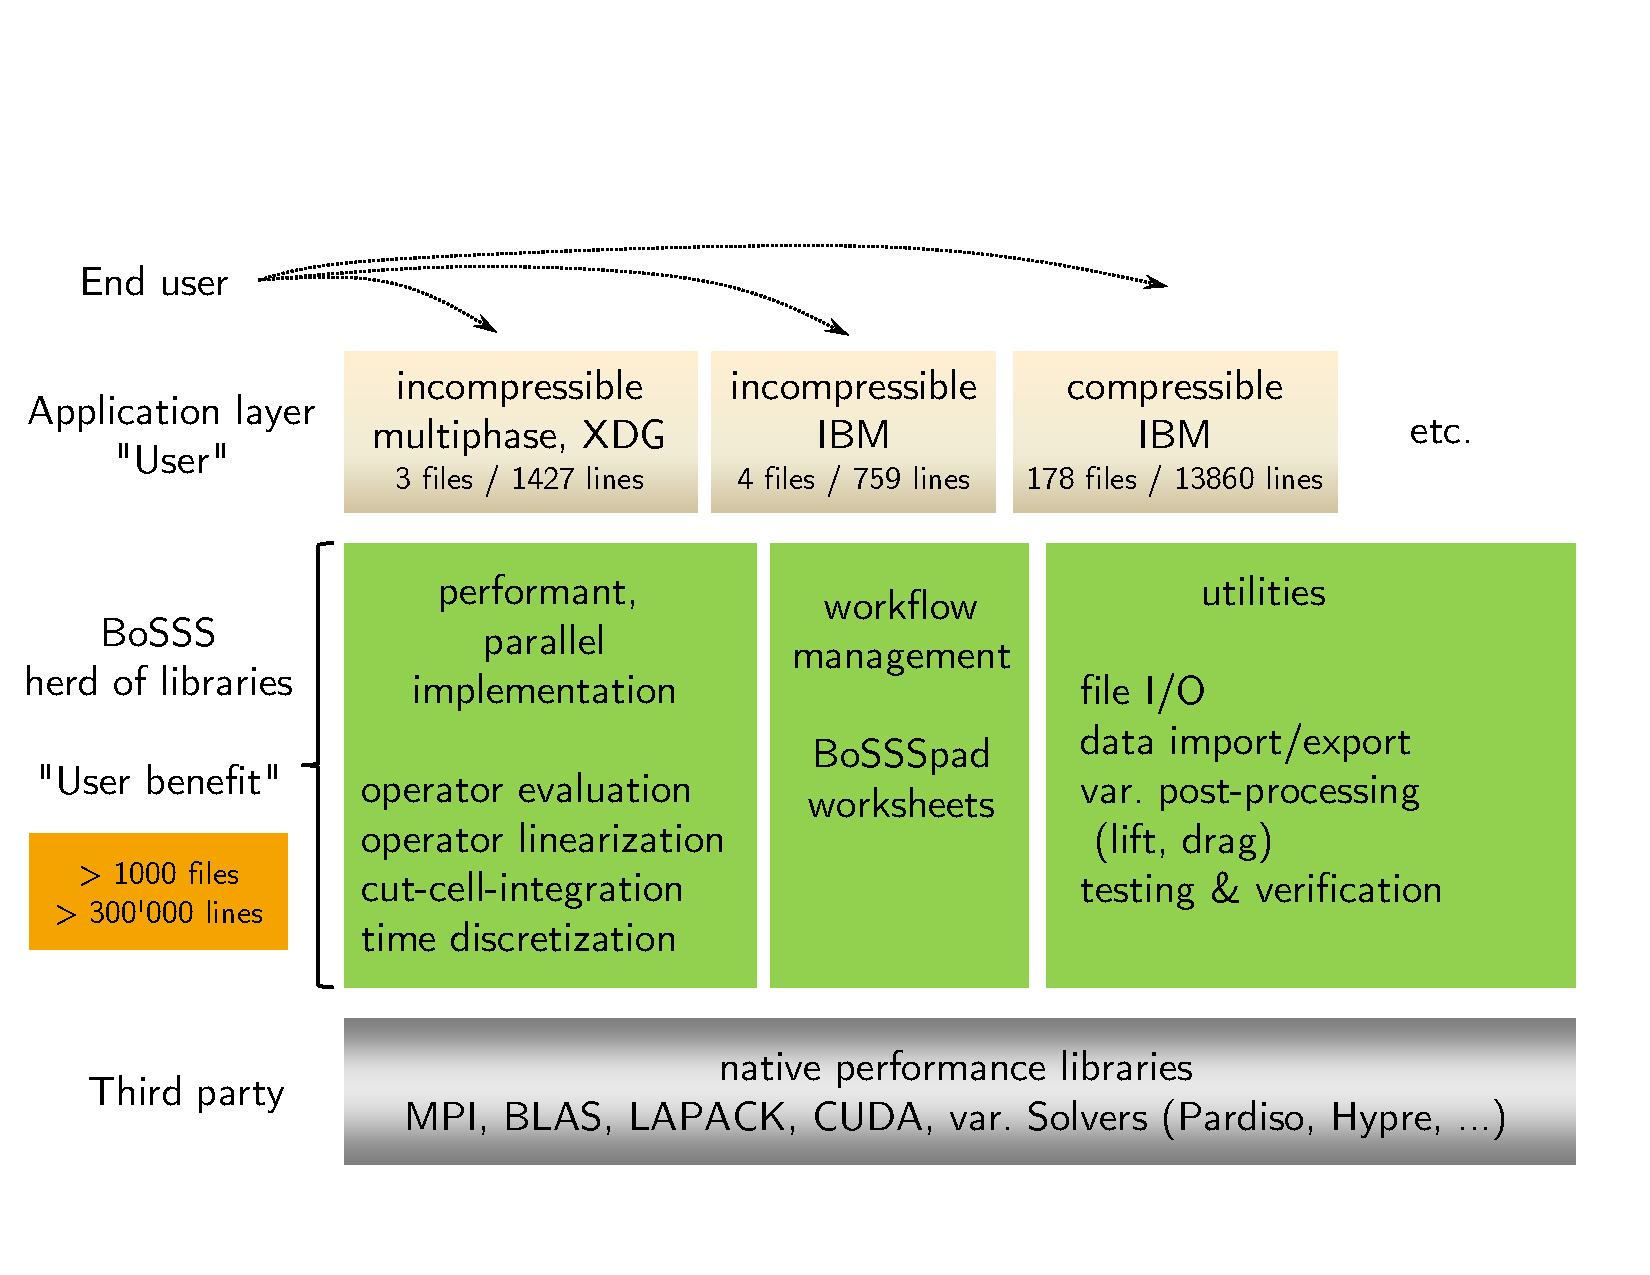
\includegraphics[width=\textwidth]{BoSSS-philosophy-1.pdf}
	\caption[Schematic representation of the structure of the BoSSS solver.]{Schematic representation of the structure of the BoSSS solver. Extracted from the BoSSS handbook \parencite{kummer2020}.}
	\label{Fig:BoSSS}
\end{figure}

